\documentclass[problem]{mcs}

\begin{pcomments}
  \pcomment{MQ_planar_isomorphism}
  \pcomment{from: S09.miniquiz-apr09}
  \pcomment{check use of \examspace[]}
\end{pcomments}

\pkeywords{
  planar_graphs
  planar_embeddings
  discrete_face
  face
  isomorphism
  recursive
}


%%%%%%%%%%%%%%%%%%%%%%%%%%%%%%%%%%%%%%%%%%%%%%%%%%%%%%%%%%%%%%%%%%%%%
% Problem starts here
%%%%%%%%%%%%%%%%%%%%%%%%%%%%%%%%%%%%%%%%%%%%%%%%%%%%%%%%%%%%%%%%%%%%%

\begin{problem} \mbox{}

\begin{center}
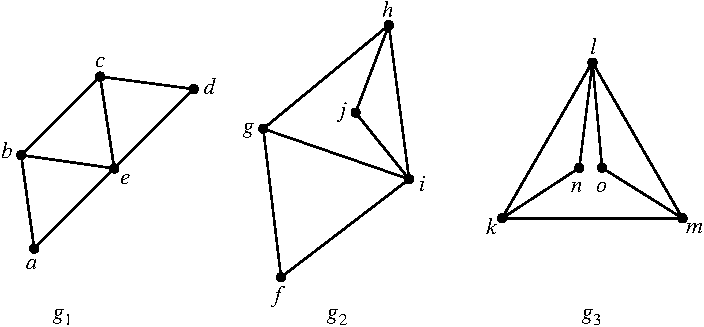
\includegraphics[width=5in]{mq4p1SP09.pdf}
\end{center}

%\vspace{-0.5in}

\bparts
\ppart[1] Describe an isomorphism between graphs $G_1$ and $G_2$,
and another isomorphism between $G_2$ and $G_3$.

\examspace[1in]

\begin{solution}

The following is a possible bijection from $G_1$ to $G_2$: \newline 
\begin{eqnarray*}
a &\longrightarrow& f, \\
b &\longrightarrow& g, \\
c &\longrightarrow& h, \\
d &\longrightarrow& j, \\
e &\longrightarrow& i \\
\end{eqnarray*}

The following is a possible bijection from $G_2$ to $G_3$: \newline
\begin{eqnarray*}
f &\longrightarrow& n, \\
g &\longrightarrow& k, \\
h &\longrightarrow& m, \\
i &\longrightarrow& l, \\
j &\longrightarrow& o
\end{eqnarray*}

\end{solution}

\ppart Why does part $(a)$ imply that there is an isomorphism between
graphs $G_1$ and $G_3$?

\examspace[1in]

\begin{solution}
The composition of an isomorphism from $G_1$ to
  $G_2$ with an isomorphism from $G_2$ to $G_3$ is an isomorphism from
  $G_1$ to $G_3$.
\end{solution}

Let $G$ and $H$ be planar graphs.  An embedding $E_G$ of $G$ is isomorphic
to an embedding $E_H$ of $H$ iff there is an isomorphism from $G$ to $H$
that also maps each face of $E_G$ to a face of $E_H$.

\ppart One of the embeddings pictured above is not isomorphic to either
of the others.  Which one?  Briefly explain why.

\examspace[1in]

\begin{solution}
  The embedding pictured in $G_2$ is not isomorphic to either of the other
  embeddings pictured because the $G_2$ embedding has a face with four
  edges, while neither of others do.
\end{solution}

\ppart Explain why all embeddings of two isomorphic planar graphs must
have the same number of faces.

\examspace[1in]

\begin{solution}
$f=2+v-e.$ 
\end{solution}

\eparts
\end{problem}

\endinput
